% !TeX program = xelatex
% !TeX encoding = UTF-8
% !TeX TXS-program:compile = txs:///xelatex | txs:///xelatex
\documentclass[aspectratio=169, table, 12pt]{beamer}
% Preamble bersama seluruh slide mata kuliah ini.
% Dipanggil dari slides/sessionXX/sessionXX.tex tepat sesudah baris
% \documentclass[aspectratio=169, table, 12pt]{beamer}
% Paket tambahan yang hanya dibutuhkan satu sesi ditulis di berkas sesi itu.

\usepackage{colortbl}
\usepackage{xcolor}
\usepackage{listings}
\usepackage{tabularx}
\usepackage{booktabs}
\usepackage{tikz}
\usepackage{pgfplots}
\pgfplotsset{compat=1.18}
\usetikzlibrary{arrows.meta, positioning, calc, fit, shapes.geometric,
	shapes.multipart, backgrounds, matrix, chains, trees}

\makeatletter
\def\input@path{{../theme/}}
\makeatother
\graphicspath{{../theme/}{../../figures/}}
\usetheme{Pradita}

\definecolor{praditagreen}{RGB}{37, 113, 71}

% Tema membuat garis tabel berwarna putih. Dikembalikan agar tabel terbaca.
\arrayrulecolor{black}
\setlength{\arrayrulewidth}{0.5pt}

\lstdefinelanguage{yaml}{
	basicstyle=\ttfamily\scriptsize,
	keywordstyle=\color{blue}\bfseries,
	commentstyle=\color{gray}\itshape,
	stringstyle=\color{red},
	showstringspaces=false,
	breaklines=true,
	frame=lines,
	numbers=none,
	backgroundcolor=\color{lightgray!10},
	tabsize=2,
	morecomment=[l]{\#}
}

\lstdefinelanguage{json}{
	basicstyle=\ttfamily\scriptsize,
	stringstyle=\color{red},
	commentstyle=\color{gray},
	breaklines=true,
	showstringspaces=false,
	tabsize=2,
	numbers=none,
	frame=lines,
	backgroundcolor=\color{lightgray!10},
	string=[s]{"}{"}
}

\lstdefinelanguage{bash}{
	keywords={},
	basicstyle=\ttfamily\scriptsize,
	ndkeywords={docker, kubectl, helm, curl, git, terraform},
	ndkeywordstyle=\color{purple}\bfseries,
	sensitive=true,
	commentstyle=\color{gray},
	numbers=none,
	breaklines=true,
	frame=lines,
	backgroundcolor=\color{lightgray!10},
	tabsize=2,
	comment=[l]{\#},
	showstringspaces=false
}

\lstdefinelanguage{http}{
	keywords={GET, POST, PUT, PATCH, DELETE, HEAD, OPTIONS, HTTP},
	basicstyle=\ttfamily\scriptsize,
	keywordstyle=\color{blue}\bfseries,
	sensitive=true,
	numbers=none,
	breaklines=true,
	frame=lines,
	backgroundcolor=\color{lightgray!10},
	tabsize=2,
	showstringspaces=false
}

\subtitle{IT40613 · Digital Platform \& API Economy}
\author{\textbf{Alfa Yohannis}}


\title{\Huge Tata Kelola API\\ \vspace{10pt} dan Regulasi Platform}
\date{Pertemuan 13}

\begin{document}
\frame{\titlepage}

\begin{frame}
  \frametitle{Isi Pertemuan}
  \vspace{14pt}
  \begin{columns}[t]
    \column{0.5\textwidth}
    {\small\tableofcontents[sections={1-6}]}

    \column{0.5\textwidth}
    {\small\tableofcontents[sections={7-12}]}
  \end{columns}
\end{frame}

\begin{frame}{\hfill}
  \centering
  \Huge{\textbf{Apotek milik sendiri\\ditaruh paling atas.\\Siapa yang boleh memutuskan?}}
\end{frame}

\section{Tujuan dan Konteks}

\begin{frame}{{\Large Tujuan Pembelajaran}}
  \vspace{10pt}
  \begin{itemize}
    \item Merancang model tata kelola API yang menjaga konsistensi tanpa memperlambat tim.
    \item Menjelaskan risiko persaingan usaha pada platform beserta regulasinya di Indonesia dan Uni Eropa.
    \item Menilai batasan regulasi terhadap rancangan platform organisasi.
  \end{itemize}
\end{frame}

\begin{frame}{{\Large Diagram Konsep Bab 13}}
  \centering
  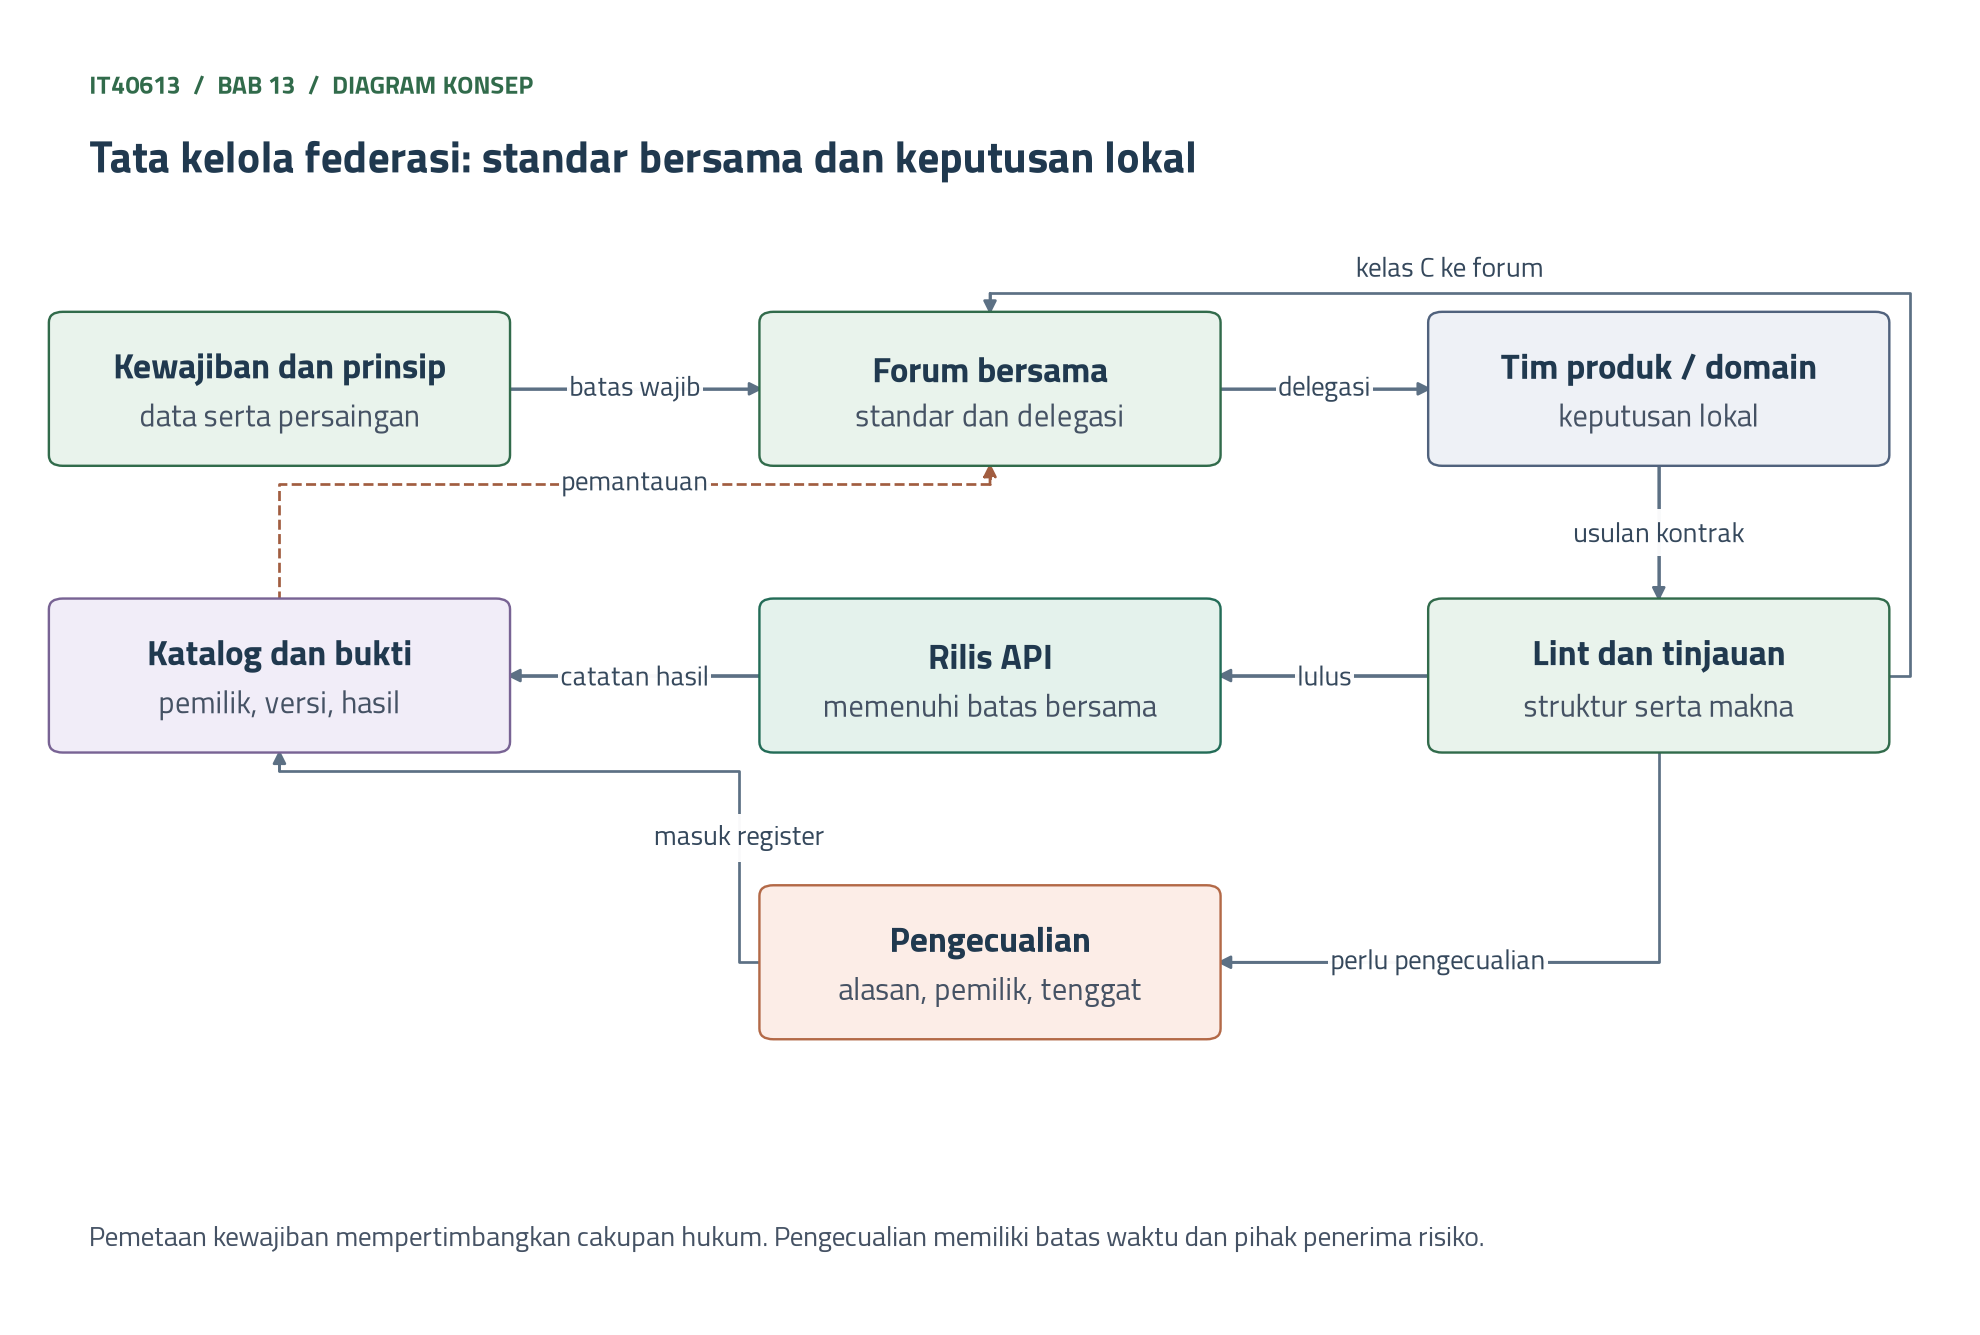
\includegraphics[width=0.96\textwidth,height=0.77\textheight,keepaspectratio]{../../figures/ch13-diagram-konsep.png}
\end{frame}

\begin{frame}{{\Large Masukan dari Bab Sebelumnya}}
  \footnotesize
  \begin{tabularx}{\textwidth}{>{\raggedright\arraybackslash}p{1.3cm} >{\raggedright\arraybackslash}X >{\raggedright\arraybackslash}p{4.3cm}}
    \hline
    \textbf{Asal} & \textbf{Keputusan yang dipakai} & \textbf{Kegunaan di sini} \\ \hline
    Bab 3 & Wasit merangkap pemain: 18 dari 58 klinik, 70 persen pemesanan & Risiko persaingan \\ \hline
    Bab 8 & API-01 sampai API-08, 12 usulan per triwulan & Isi katalog, jumlah usulan \\ \hline
    Bab 9 & Kontrak API-01 dengan 4 operasi & Sumber panduan gaya \\ \hline
    Bab 10 & Masa transisi 6 bulan, sisa cadangan 120 jam & Tenggat pengecualian \\ \hline
    Bab 11 & SLA 99,0 persen, SLO 99,4 persen & Janji di katalog \\ \hline
    Bab 12 & Paket berjenjang, Rp1,44 miliar per tahun & Batas meniru DMA \\ \hline
  \end{tabularx}

  \vspace{8pt}
  \small Tetap dipakai: 20 sambungan aktif, Rp45 juta per antarmuka, tarif Rp60.000 per jam, lapisan bersama Rp300 juta per tahun, 40 klinik mitra, kuota 300 per hari per klinik.
\end{frame}

\section{Tata Kelola sebagai Pemungkin}

\begin{frame}{{\Large Tata Kelola API sebagai Pemungkin}}
  \vspace{8pt}
  \begin{itemize}
    \item Menetapkan hak keputusan, standar minimum, bukti persetujuan, dan pengecualian.
    \item Tujuannya menjaga kemampuan berubah dengan konsisten.
    \item Pemeriksaan disesuaikan dengan risiko.
    \item Pemilik keputusan dan waktu layanan forum harus terlihat.
    \item COBIT dan tata kelola umum dibahas rinci di IT40813.
  \end{itemize}
  \vspace{6pt}
  {\small Analogi: aturan lalu lintas memudahkan perjalanan, tanpa meminta izin di setiap tikungan.}
\end{frame}

\begin{frame}{{\Large Dua Contoh Berangka}}
  \vspace{8pt}
  \begin{itemize}
    \item 48 usulan API-01 per tahun menunggu forum bulanan: 480 hari-usulan.
    \item Misalkan dibagi kelas A, B, C: 30, 14, dan 4 usulan: 112 hari-usulan.
    \item Tunggu turun 368 hari-usulan, atau sekitar 77 persen.
    \item Misalkan 5 format galat: 40 klinik, 4 format tambahan, 4 jam.
    \item Beban 640 jam, atau Rp38,4 juta, jatuh pada mitra.
  \end{itemize}
\end{frame}

\begin{frame}{{\Large Peta Keputusan: Jalur Menurut Risiko}}
  \centering
  \eadiagram{../../figures/ch13-peta-keputusan.tex}
\end{frame}

\begin{frame}{{\Large Yang Sering Tertukar: Tata Kelola dan Birokrasi}}
  \vspace{8pt}
  \begin{itemize}
    \item Tata kelola memperjelas siapa memutuskan dan bukti apa yang diminta.
    \item Birokrasi menambah tanda tangan tanpa mengubah keputusan.
    \item Uji: bila satu tanda tangan dihapus, risiko apa yang tidak lagi diperiksa?
    \item Forum memeriksa contoh acak 10 persen, karena kelas dapat dimanipulasi.
    \item Waktu layanan forum adalah janji, sama seperti SLO.
  \end{itemize}
\end{frame}

\section{Model Tata Kelola}

\begin{frame}{{\Large Terpusat, Terdistribusi, dan Federasi}}
  \centering
  \eadiagram{../../figures/ch13-model-federasi.tex}
\end{frame}

\begin{frame}{{\Large Tiga Model pada 48 Usulan}}
  \footnotesize
  \begin{tabularx}{\textwidth}{>{\raggedright\arraybackslash}p{2.3cm} >{\raggedright\arraybackslash}p{2.4cm} >{\raggedright\arraybackslash}p{1.9cm} >{\raggedright\arraybackslash}X}
    \hline
    \textbf{Model} & \textbf{Tunggu} & \textbf{Biaya} & \textbf{Kelemahan utama} \\ \hline
    Terpusat & 480 hari-usulan & Rp7,2 juta & Antrean, tim pusat tidak mengenal kelima SIMRS \\ \hline
    Terdistribusi & 48 hari-usulan & Rp1,44 juta & Fragmentasi, klinik memikul Rp38,4 juta \\ \hline
    Federasi & 112 hari-usulan & Rp9,78 juta & Perlu forum yang benar-benar memutuskan \\ \hline
  \end{tabularx}

  \vspace{8pt}
  \small Federasi bukan yang termurah. Keunggulannya terletak pada kombinasi tunggu yang pendek dan beban yang tidak dilempar ke klinik.

  \vspace{4pt}
  \small Analogi: cabang berbagi aturan keselamatan, tetapi mengatur jam buka sendiri.
\end{frame}

\begin{frame}{{\Large Hak Keputusan pada Federasi}}
  \footnotesize
  \begin{tabularx}{\textwidth}{>{\raggedright\arraybackslash}p{3.0cm} >{\raggedright\arraybackslash}X >{\raggedright\arraybackslash}X >{\raggedright\arraybackslash}X}
    \hline
    \textbf{Keputusan} & \textbf{Forum bersama} & \textbf{Pemilik produk} & \textbf{Tim integrasi} \\ \hline
    Panduan gaya, format galat & Memutuskan & Memberi masukan & Mengusulkan \\ \hline
    Masa transisi 6 bulan & Memutuskan & Menerima biaya & Menerapkan \\ \hline
    Bidang data baru & Memutuskan bila kelas C & Mengusulkan tujuan & Menilai dampak kontrak \\ \hline
    Isi API-01, prioritas & Tidak terlibat & Memutuskan & Memberi perkiraan \\ \hline
    Adaptor SIMRS & Tidak terlibat & Dikabari & Memutuskan bersama tim rumah sakit \\ \hline
  \end{tabularx}

  \vspace{8pt}
  \small Keamanan dan petugas pelindungan data meninjau, dan boleh memangkas masa transisi saat kerentanan serius.
\end{frame}

\begin{frame}{{\Large Berapa Biaya Tata Kelola?}}
  \vspace{8pt}
  \begin{itemize}
    \item Tahun pertama: 163 jam berjalan, 80 jam panduan, 80 jam pendampingan.
    \item Jumlahnya 323 jam, atau Rp19,38 juta.
    \item Sisa pagu lapisan bersama Rp300 juta hanya Rp1,2 juta.
    \item Rp19,38 juta adalah kapasitas, bukan kas, bila dikerjakan karyawan yang sudah digaji.
    \item Paling banyak 227 jam, padahal cadangan 1.080 jam Bab 8 tinggal 60 jam: kurang 167 jam, dijumlahkan di Bab 14.
  \end{itemize}
\end{frame}

\begin{frame}{{\Large Kasus Medikara: Forum Bersama}}
  \vspace{6pt}
  \begin{itemize}
    \item Misalkan 5 anggota: rawat jalan, keamanan, pelindungan data, kemitraan, tim integrasi.
    \item Format galat dan identitas klien menjadi standar bersama.
    \item Rumah sakit dengan SIMRS tertua: pengecualian 6 bulan, adaptor 40 jam, Rp2,4 juta.
    \item API-08 belum masuk antrean rilis sebelum ada pemilik.
    \item Ditinjau sesudah 6 bulan, dengan dua pemicu tertulis.
  \end{itemize}
  \vspace{4pt}
  {\small Usulan belum menjadi keputusan sebelum pemilik menerima konsekuensinya.}
\end{frame}

\section{Panduan Gaya dan Pemeriksaan}

\begin{frame}{{\Large Panduan Gaya dan Bukti Pendukungnya}}
  \vspace{6pt}
  \begin{itemize}
    \item Panduan gaya menetapkan penamaan, galat, pembagian halaman, dan keamanan.
    \item Macvean dkk.: API Google yang tumbuh cepat menghasilkan ketidakkonsistenan. Google memakai tinjauan ringan dan terdistribusi.
    \item Bogner dkk.: 105 peserta, 12 aturan. Pelanggaran memperburuk pemahaman pada 11 aturan.
    \item Zalando: MUST, SHOULD, MAY. Dimiliki API Guild, diperiksa \textit{linter}.
    \item Google AIP: status \textit{Draft}, \textit{Reviewing}, dan \textit{Approved}.
  \end{itemize}
\end{frame}

\begin{frame}{{\Large Panduan Gaya Contoh Medikara}}
  \footnotesize
  \begin{tabularx}{\textwidth}{>{\raggedright\arraybackslash}p{1.7cm} >{\raggedright\arraybackslash}p{2.2cm} >{\raggedright\arraybackslash}X >{\raggedright\arraybackslash}p{1.9cm}}
    \hline
    \textbf{Butir} & \textbf{Tingkat} & \textbf{Isi} & \textbf{Pemeriksa} \\ \hline
    GAYA-01 & WAJIB & Jalur huruf kecil dan tanda hubung & Mesin \\ \hline
    GAYA-02 & WAJIB & \texttt{operationId} dan \texttt{summary} & Mesin \\ \hline
    GAYA-03 & WAJIB & \texttt{security} dan \textit{scope} & Mesin \\ \hline
    GAYA-04 & WAJIB & Galat memakai \texttt{application/problem+json} & Mesin \\ \hline
    GAYA-05 & WAJIB & POST menerima \texttt{Idempotency-Key} & Mesin \\ \hline
    GAYA-06 & SEBAIKNYA & Daftar punya parameter \texttt{batas} & Mesin \\ \hline
    GAYA-07 & WAJIB & Setiap bidang punya tujuan tertulis & Manusia \\ \hline
    GAYA-08 & WAJIB & Hak atas objek diuji & Manusia \\ \hline
  \end{tabularx}
\end{frame}

\begin{frame}{{\Large Dua Contoh Berangka}}
  \vspace{8pt}
  \begin{itemize}
    \item Kontrak API-01: 4 operasi, 0 temuan. Kontrak contoh: 2 operasi, 10 temuan.
    \item Insiden Bab 6 memakai token sah: kontrak seperti itu dapat lulus \textit{lint}.
    \item Misalkan manual 48 menit per usulan, 18 usulan: 14,4 jam, Rp864.000 per tahun.
    \item Pemasangan pemeriksa 16 jam, Rp960.000: impas sesudah lebih dari setahun.
    \item Manfaat utamanya hasil yang sama, dan tinjauan fokus pada makna.
  \end{itemize}
  \vspace{4pt}
  {\small Analogi: pemeriksa ejaan membantu penyunting, tetapi tidak membuktikan isi tulisan benar.}
\end{frame}

\begin{frame}{{\Large Yang Sering Tertukar: Lint dan Tinjauan}}
  \footnotesize
  \begin{tabularx}{\textwidth}{>{\raggedright\arraybackslash}p{2.6cm} >{\raggedright\arraybackslash}X >{\raggedright\arraybackslash}X}
    \hline
    \textbf{Pemeriksaan} & \textbf{Yang dinilai} & \textbf{Yang tidak dapat dinilai} \\ \hline
    \textit{Lint} & Nama jalur, kelengkapan, format galat & Arti bidang, hak atas objek, dampak pada pasien \\ \hline
    Tinjauan desain & Arti status, data minimum, kebutuhan klinik & Konsistensi ribuan baris secara andal \\ \hline
    Pengecualian & Penyimpangan yang disengaja dan beralasan & Penyimpangan yang tidak dilaporkan \\ \hline
  \end{tabularx}

  \vspace{8pt}
  \small Misalkan 2 pengecualian baru per triwulan. Tanpa tenggat: 24 aktif sesudah 3 tahun. Dengan tenggat 6 bulan: paling banyak 4.
\end{frame}

\section{Katalog dan Kepemilikan}

\begin{frame}{{\Large Katalog dan Kepemilikan API}}
  \vspace{8pt}
  \begin{itemize}
    \item Katalog mencatat pemilik, versi, status, kelas data, kontrak, dan hasil uji.
    \item Pemilik berarti satu jabatan yang menerima konsekuensi.
    \item OWASP API9: inventaris yang lemah adalah risiko tersendiri.
    \item INT-10: 12 dari 100 sambungan tanpa pemilik. Penelusuran 24 jam, Rp1,44 juta.
    \item Portal melayani pemakai, sedangkan katalog melayani pengelola.
  \end{itemize}
  \vspace{4pt}
  {\small Analogi: alat rumah sakit tanpa catatan kalibrasi tidak dipakai pada pasien.}
\end{frame}

\begin{frame}{{\Large Tiga Baris Katalog Contoh}}
  \footnotesize
  \begin{tabularx}{\textwidth}{>{\raggedright\arraybackslash}p{2.5cm} >{\raggedright\arraybackslash}p{2.9cm} >{\raggedright\arraybackslash}X}
    \hline
    \textbf{API} & \textbf{Pemilik} & \textbf{Janji dan bukti} \\ \hline
    API-01 Janji Temu & Manajer Layanan Rawat Jalan & Kontrak 1.0.0, SLA 99,0 persen, SLO 99,4 persen, masa transisi 6 bulan \\ \hline
    API-02 Hasil & Manajer Laboratorium & Belum ada kontrak. Kelas C, penilaian dampak lebih dahulu \\ \hline
    API-08 Resep & Belum ada & Tidak boleh masuk antrean rilis sebelum ada pemilik \\ \hline
  \end{tabularx}

  \vspace{8pt}
  \small Dari 8 baris, 7 punya pemilik dan 1 punya kontrak. Forum membaca empat angka tiap triwulan: API tanpa pemilik, pengecualian lewat tenggat, tunggu kelas C, dan API di luar katalog.
\end{frame}

\section{Ekosistem Mitra}

\begin{frame}{{\Large Tata Kelola Ekosistem Mitra}}
  \vspace{6pt}
  \begin{itemize}
    \item Aturan masuk: kriteria terbuka dan dapat diverifikasi.
    \item Kurasi: mutu dinilai dengan ukuran tertulis.
    \item Sanksi: bertahap, berbasis bukti, dengan jalur keberatan.
    \item Misalkan 15 apotek daring: 60 jam, Rp3,6 juta, 3 ditolak dengan alasan tertulis.
    \item Lab 400 dari 1.100 pemeriksaan: dicabut mendadak, dua lab lain naik 57 persen.
  \end{itemize}
  \vspace{4pt}
  {\small Analogi: pengelola pasar memerlukan kriteria tempat usaha dan jalur keberatan.}
\end{frame}

\begin{frame}{{\Large Tangga Sanksi Bagi Mitra}}
  \centering
  \eadiagram{../../figures/ch13-tangga-sanksi.tex}
\end{frame}

\begin{frame}{{\Large Yang Sering Tertukar: Kurasi dan Sanksi}}
  \vspace{8pt}
  \begin{itemize}
    \item Kurasi menilai siapa tampil dan urutannya, dengan ukuran yang berlaku bagi semua.
    \item Sanksi menanggapi pelanggaran atas aturan.
    \item Menurunkan urutan diam-diam sebagai hukuman menutup jalur keberatan.
    \item Aturan yang sama berlaku bagi 18 klinik dan 12 apotek milik Medikara.
    \item Keadaan darurat: Kepala Keamanan Informasi boleh menangguhkan lebih dahulu.
  \end{itemize}
\end{frame}

\section{Persaingan Usaha}

\begin{frame}{{\Large Persaingan Usaha pada Platform}}
  \vspace{6pt}
  \begin{itemize}
    \item Posisi dominan tidak otomatis melanggar. Penyalahgunaannya bermasalah.
    \item UU 5/1999 dan KPPU. Pasal 25: 50 persen, atau 75 persen untuk 2 sampai 3 pelaku.
    \item \textit{Self-preferencing}: platform mengutamakan produknya sendiri.
    \item Farronato dkk.: merek Amazon ditempatkan lebih tinggi daripada produk serupa.
    \item Hagiu dkk.: aturan main dapat lebih baik daripada larangan berjualan.
  \end{itemize}
  \vspace{4pt}
  {\small Analogi: pemilik pusat belanja yang juga berdagang.}
\end{frame}

\begin{frame}{{\Large Empat Langkah Menilai Risiko}}
  \centering
  \eadiagram{../../figures/ch13-uji-persaingan.tex}
\end{frame}

\begin{frame}{{\Large Dua Contoh Berangka}}
  \vspace{8pt}
  \begin{itemize}
    \item Misalkan 12 dari 1.200 apotek di wilayah layanan: 1 persen.
    \item Pada definisi sempit, tebus di Medikara+: 76 persen. Ambangnya 50 persen.
    \item Definisi pasar menentukan kesimpulan, sehingga bukan kebiasaan tim.
    \item Bab 3: 18 dari 58 klinik, atau 31 persen, menerima 70 persen pemesanan.
    \item Selisih 39 poin belum membuktikan perlakuan istimewa: bandingkan yang serupa.
  \end{itemize}
\end{frame}

\begin{frame}{{\Large Perkara Google Play Billing}}
  \footnotesize
  \begin{tabularx}{\textwidth}{>{\raggedright\arraybackslash}p{2.7cm} >{\raggedright\arraybackslash}X}
    \hline
    \textbf{Unsur} & \textbf{Isi menurut siaran pers dan berita} \\ \hline
    Perilaku & Wajib memakai Google Play Billing mulai 1 Juni 2022, pembayaran lain tidak diperkenankan \\ \hline
    Biaya, penolak & 15 sampai 30 persen. Aplikasi penolak dapat dihapus \\ \hline
    Pasal terbukti & Pasal 17 dan Pasal 25 ayat (1) huruf b, 21 Januari 2025 \\ \hline
    Sanksi, perintah & Denda Rp202,5 miliar, buka UCB, pengurangan biaya minimal 5 persen selama 1 tahun \\ \hline
    Upaya hukum & Pengadilan Niaga 19 Juni 2025. Mahkamah Agung 10 Maret 2026 \\ \hline
  \end{tabularx}

  \vspace{6pt}
  \small Sumber sekunder. Teks putusan belum dibaca. Fakta perkara ini tidak otomatis berlaku pada kasus lain.
\end{frame}

\begin{frame}{{\Large Empat Tuas Pemilik Platform}}
  \footnotesize
  \begin{tabularx}{\textwidth}{>{\raggedright\arraybackslash}p{2.4cm} >{\raggedright\arraybackslash}X >{\raggedright\arraybackslash}X}
    \hline
    \textbf{Tuas} & \textbf{Bentuk bermasalah} & \textbf{Rancangan yang dapat dijelaskan} \\ \hline
    Urutan tampil & Milik sendiri selalu teratas & Kriteria tertulis, berversi, dengan label \\ \hline
    Kuota dan akses & Klinik sendiri tanpa batas, mitra 300 per hari & Satu aturan kuota \\ \hline
    Data & Data mitra dibaca klinik sendiri & Akses dipisahkan \\ \hline
    Pembayaran & Mitra wajib memakai pembayaran Medikara & Pilihan terbuka, biaya diumumkan \\ \hline
  \end{tabularx}

  \vspace{8pt}
  \small Tiap tuas sah dipakai. Yang dinilai adalah alasan, keterbukaan, dan akibatnya.
\end{frame}

\begin{frame}{{\Large Kasus Medikara: Audit Urutan Klinik}}
  \vspace{6pt}
  \begin{itemize}
    \item Misalkan wakil klinik mitra mempertanyakan angka 70 persen.
    \item 200 pencarian sintetis: klinik milik Medikara pertama pada 62, atau 31 persen.
    \item Pada contoh itu, urutan mengikuti kriteria.
    \item Hasil ini bukan bukti tidak ada pelanggaran: pasar dan akibat belum dinilai.
    \item Kriteria diberi versi. Audit tiap triwulan: Rp960.000, atau Rp3,84 juta per tahun.
  \end{itemize}
\end{frame}

\section{Regulasi Uni Eropa}

\begin{frame}{{\Large DMA dan Kewajiban Gatekeeper}}
  \vspace{6pt}
  \begin{itemize}
    \item Berlaku bagi perusahaan yang ditunjuk: tujuh, dengan 23 layanan platform inti.
    \item Omzet EUR 7,5 miliar, atau nilai pasar EUR 75 miliar, di minimal tiga negara.
    \item 45 juta pengguna akhir per bulan dan 10.000 pengguna bisnis per tahun.
    \item Denda sampai 10 persen omzet dunia, atau 20 persen bila berulang.
    \item Pertimbangan 11: berlaku terlepas dari dampak perilaku pada pasar.
  \end{itemize}
  \vspace{4pt}
  {\small Medikara: ambang 37,5 kali kunjungan dan 250 kali klinik mitra. Tidak berlaku, hanya pembanding.}
\end{frame}

\begin{frame}{{\Large Empat Kewajiban dan Pembacaannya}}
  \footnotesize
  \begin{tabularx}{\textwidth}{>{\raggedright\arraybackslash}p{1.7cm} >{\raggedright\arraybackslash}X >{\raggedright\arraybackslash}X >{\raggedright\arraybackslash}p{1.8cm}}
    \hline
    \textbf{Pasal} & \textbf{Isi pokok} & \textbf{Prinsip pada Medikara} & \textbf{Keputusan} \\ \hline
    5 ayat (2) & Tidak menggabungkan data antarlayanan tanpa persetujuan & Data mitra tidak dibuka bagi klinik sendiri & Ditiru \\ \hline
    6 ayat (5) & Tidak mengutamakan layanan sendiri dalam pemeringkatan & Kriteria urutan tertulis & Ditiru \\ \hline
    6 ayat (7) & Interoperabilitas gratis & API yang sama, lewat paket berbayar & Sebagian \\ \hline
    6 ayat (12) & Syarat akses yang adil, dengan penyelesaian sengketa & Syarat terbit, jalur keberatan & Ditiru \\ \hline
  \end{tabularx}

  \vspace{6pt}
  \small Akses gratis ditolak dengan sadar, karena akan menghapus Rp1,44 miliar per tahun.
\end{frame}

\begin{frame}{{\Large Penegakan DMA Sampai Saat Diakses}}
  \footnotesize
  \begin{tabularx}{\textwidth}{>{\raggedright\arraybackslash}p{2.4cm} >{\raggedright\arraybackslash}p{1.95cm} >{\raggedright\arraybackslash}X >{\raggedright\arraybackslash}p{2.1cm}}
    \hline
    \textbf{Tanggal} & \textbf{Perusahaan} & \textbf{Pelanggaran} & \textbf{Denda} \\ \hline
    23 April 2025 & Apple & Membatasi pengarahan ke tawaran di luar App Store & EUR 500 juta \\ \hline
    23 April 2025 & Meta & ``Setuju atau bayar'' & EUR 200 juta \\ \hline
    23 Juli 2026 & Google & Mengutamakan layanan sendiri pada Search & EUR 460 juta \\ \hline
    23 Juli 2026 & Google & Membatasi pengarahan ke luar Google Play & EUR 430 juta \\ \hline
  \end{tabularx}

  \vspace{8pt}
  \small Siaran pers Komisi Eropa. Status banding perlu diperiksa saat dipakai. Google diberi 60 hari untuk mematuhi.
\end{frame}

\section{Batas Data dan Sektor}

\begin{frame}{{\Large Batas Pemakaian Data}}
  \vspace{6pt}
  \begin{itemize}
    \item Data dibatasi menurut tujuan, dasar pemrosesan, peran, dan masa kebutuhan.
    \item Persetujuan hanya satu dari enam dasar pemrosesan.
    \item PP 33/2026 berlaku 16 Januari 2027. Naskah resmi belum diperoleh: salinan pihak ketiga, hanya dipantau.
    \item Misalkan 4 bidang menjadi 10 bidang: 1.240 rekam, 4.960 menjadi 12.400 butir.
    \item Klinik keluar: token mati 15 menit, 35 rujukan diselesaikan dalam 30 hari.
  \end{itemize}
  \vspace{4pt}
  {\small Analogi: meminjam dokumen untuk satu urusan bukan izin untuk semua urusan.}
\end{frame}

\begin{frame}{{\Large Lapis Batasan pada Rancangan}}
  \centering
  \eadiagram{../../figures/ch13-lapis-batasan.tex}
\end{frame}

\begin{frame}{{\Large Pasal dan Akibatnya pada API}}
  \footnotesize
  \begin{tabularx}{\textwidth}{>{\raggedright\arraybackslash}p{3.0cm} >{\raggedright\arraybackslash}X >{\raggedright\arraybackslash}X}
    \hline
    \textbf{Sumber} & \textbf{Isi pokok} & \textbf{Akibat} \\ \hline
    PP 33/2026 Pasal 58, 59 & Data tidak melebihi kebutuhan tujuan & GAYA-07 \\ \hline
    PP 33/2026 Pasal 14, 15 & Isi minimum perjanjian prosesor & Tinjau perjanjian vendor \\ \hline
    PP 33/2026 Pasal 120, 121 & Penilaian dampak sebelum pemrosesan berisiko tinggi & API-02 kelas C \\ \hline
    PP 33/2026 Pasal 185 & Denda sampai 2 persen pendapatan tahunan & Pengendali dan prosesor \\ \hline
    Permenkes 24/2022 Pasal 32 & Kerahasiaan isi rekam medis & API janji temu tidak membukanya \\ \hline
  \end{tabularx}

  \vspace{6pt}
  \small Pasal PP 33/2026 dari salinan pihak ketiga. Tata kelola pelindungan data secara rinci dibahas di IT40813.
\end{frame}

\begin{frame}{{\Large Kasus Medikara: Batasan pada API-02}}
  \vspace{6pt}
  \begin{itemize}
    \item Hasil pemeriksaan adalah data spesifik, sehingga masuk kelas C.
    \item Penilaian dampak dilakukan sebelum pemrosesan, walau API-02 baru rilis Oktober 2028.
    \item Misalkan 40 jam, atau Rp2,4 juta, dibayar sebelum kontrak ditulis.
    \item Hasilnya dapat mengubah bidang pada kontrak.
    \item Bidang \texttt{spesialis} pada API-01: pertanyaan terbuka bagi penasihat hukum.
  \end{itemize}
\end{frame}

\section{Aktivitas}

\begin{frame}{{\Large Aktivitas: Model Tata Kelola dan Batasan Regulasi}}
  \vspace{4pt}
  \begin{itemize}
    \item Tujuan: model tata kelola API dan daftar batasan regulasi untuk tonggak C4.
    \item Anggota hukum dan bisnis: batasan persaingan, data, dan sektor.
    \item Anggota teknis: aturan pemeriksaan otomatis untuk panduan gaya.
    \item Tim: hak keputusan, kelas perubahan, titik pemeriksaan, pengecualian.
    \item Kaitan: C4 Peta Jalan dan Tata Kelola. Kriteria: 25, 30, 30, dan 15 persen.
  \end{itemize}
  \vspace{4pt}
  {\footnotesize Berkas pendukung: \berkas{sources/chapter13/README.md}. Pakai data sintetis, atau data berizin yang dianonimkan. Opsional: dua aturan Spectral.}
\end{frame}

\section{Ringkasan}

\begin{frame}{{\Large Ringkasan}}
  \vspace{4pt}
  \begin{itemize}
    \item Tata kelola yang baik membuat keputusan terlihat, bukan menambah rapat.
    \item Federasi membagi batas bersama dan keputusan lokal: 112 hari-usulan, Rp9,78 juta.
    \item \textit{Lint} memeriksa bentuk, tinjauan menilai makna, dan pengecualian punya tenggat.
    \item Pangsa 1 atau 76 persen bergantung pada definisi pasar.
    \item DMA hanya pembanding. UU 27/2022 membatasi rancangan, PP 33/2026 dipantau.
  \end{itemize}
\end{frame}

\section{Latihan}

\begin{frame}{{\Large Latihan}}
  \vspace{8pt}
  \begin{enumerate}
    \item Jelaskan perbedaan tata kelola API terpusat dan federasi, lalu tentukan model yang cocok bagi Medikara dengan lima rumah sakit hasil akuisisi.
    \item Misalkan Medikara berencana menampilkan apotek miliknya di urutan teratas aplikasi Medikara+, di atas apotek mitra. Analisis risikonya dari sudut persaingan usaha.
    \item Ambil satu kewajiban \textit{gatekeeper} dalam DMA, lalu jelaskan apakah prinsipnya relevan bagi platform kesehatan di Indonesia.
  \end{enumerate}
  \vspace{6pt}
  {\small Setiap latihan punya tabel contoh dan lembar isian pada Bab 13.}
\end{frame}

\end{document}
